\documentclass[letterpaper,11pt]{article}



\usepackage[utf8]{inputenc}
\usepackage[letterpaper,hmargin=1in,vmargin=1in,footskip=36pt]{geometry}
\sloppy

\usepackage{cite} 

\usepackage{amsmath,amsthm}
\usepackage{amsfonts,amssymb}

\usepackage{paralist}

\newtheorem{theorem}{Theorem}
\newtheorem{lemma}{Lemma}
\newtheorem{prop}{Proposition}
\newtheorem{cor}{Corollary}
\newtheorem{definition}{Definition}
\newtheorem{observation}{Observation}

\usepackage[font=small,labelfont=bf]{caption}

\usepackage{graphicx}
\usepackage{tikz}
\usetikzlibrary{chains,fit,shapes,decorations.pathmorphing,arrows}
\usepackage{xcolor,color}

\usepackage{multirow}
\usepackage{tabularx,booktabs}
\newcolumntype{Y}{>{\raggedright\arraybackslash}X}
\newcolumntype{Z}{>{\centering\arraybackslash}X}

\usepackage{algorithmic}
\usepackage{algorithm}
\renewcommand{\algorithmicrequire}{\textbf{Input:}}
\newcommand{\EXPECT}[1]{\mathbb{E}\left[#1\right]}

\newcommand{\bbalgo}{GA}

\usepackage{xspace}

\newcommand{\EDF}{\ensuremath{\mathsf{EDF}}\xspace}
\newcommand{\LLF}{\ensuremath{\mathsf{LLF}}\xspace}
\newcommand{\OPT}{\ensuremath{\mathsf{OPT}}\xspace}
\newcommand{\Earlyfit}{\ensuremath{\mathsf{EarlyFit}}\xspace}
\newcommand{\Mediumfit}{\ensuremath{\mathsf{MediumFit}}\xspace}
\newcommand{\A}{\ensuremath{\mathsf{A}}\xspace}
\newcommand{\double}{{\sf Double}\xspace}


\newcommand{\OO}{\ensuremath{\mathcal{O}}}

\newcommand{\II}{\ensuremath{\mathcal{I}}}

\newcommand{\N}{\ensuremath{\mathbb{N}}}
\newcommand{\R}{\ensuremath{\mathbb{R}}}
\newcommand{\Q}{\ensuremath{\mathbb{Q}}}
\newcommand{\eps}{\varepsilon}

\DeclareMathOperator{\ex}{ex}

\usepackage[textsize=tiny,textwidth=2cm,shadow,color=green]{todonotes}
\newcommand{\nic}[1]{\todo[color=green]{N: #1}}
\newcommand{\kev}[1]{\todo[color=yellow]{K: #1}}
\newcommand{\lin}[1]{\todo[color=pink]{L: #1}}
\newcommand{\red}[1]{\textcolor{red}{#1}}

\title{New Results on Online Resource Minimization\thanks{This research was supported by the
    German Science Foundation (DFG) under contract  ME 3825/1. The
    third author was supported by the DFG within the research
    training group `Methods for Discrete Structures' (GRK 1408).}}

\author{
Lin Chen\thanks{Technische Universit\"at M\"unchen, Zentrum
   f\"ur Mathematik, Garching, Germany. Email:
   \texttt{nmegow@ma.tum.de}, \texttt{chenlin198662@gmail.com}.}
 \and Nicole Megow\footnotemark[2]  \and Kevin Schewior\thanks{Technische Universit\"at Berlin, Institut f\"ur
  Mathematik, Berlin, Germany. Email:
  \texttt{schewior@math.tu-berlin.de}.}}

\date{\today}

\begin{document}


\maketitle
\thispagestyle{empty}

\begin{abstract}
We consider the online resource minimization problem in which jobs
with hard deadlines arrive online over time at their release
dates. The task is to determine a feasible schedule on a minimum
number of machines. 

We rigorously study this problem and derive various algorithms with small constant competitive ratios for interesting restricted problem variants. As the most important special case, we consider scheduling jobs with
agreeable deadlines. We provide the first constant-ratio competitive
algorithm for the non-preemptive setting, which is of particular
interest with regard to the known strong lower bound of~ for the
general problem. For the preemptive setting, we show that the natural
algorithm \LLF achieves a constant ratio for agreeable jobs, while in general it has a lower bound of .

We also give an -competitive algorithm for the general preemptive problem, which improves upon a known -competitive algorithm. Our algorithm maintains a dynamic partition of the job set into loose and tight jobs and schedules each (temporal) subset individually on separate sets of machines. The key is a characterization of how the decrease in the relative laxity of jobs influences the optimum number of machines. To achieve this we derive  a compact expression of the optimum value, which might be of independent interest. We complement the general algorithmic result by showing lower bounds that rule out that other known algorithms may yield a similar performance~guarantee.

\end{abstract}

\clearpage
\setcounter{page}{1}

\section{Introduction} Minimizing the resource usage is a key  to the
achievement of economic, environmental or societal goals.
We consider the fundamental problem of minimizing the number of
machines that is necessary for feasibly scheduling jobs with
release dates and hard deadlines. We consider the online variant of this problem in which every job
becomes known to the online algorithm only at its release date. We
denote this problem as {\em online machine minimization problem}. We also
consider a {\em semi-online} variant in which we give the
online algorithm slightly more information by giving the optimal
number of machines as part of the input.

We develop several algorithms for preemptive and non-preemptive problem variants, and evaluate
their performance by  the competitive ratio, a widely-used measure that
compares the solution value of an online algorithm with an optimal
offline value. We derive the first constant-competitive 
algorithms for certain variants of (semi-)online machine minimization
and improve several others. As a major special case, we consider online deadline
scheduling with {\em agreeable deadlines}, i.e., when the order of deadlines for all jobs coincides with the order of
their release dates.  We give the first constant-competitive algorithm for scheduling agreeable jobs non-preemptively,
which contrasts to the strong lower bound of  for the general
problem~\cite{Saha13}. We also prove that for the preemptive scheduling problem, one of the most natural algorithms called {\em Least Laxity First} (\LLF) achieves a constant ratio for agreeable jobs, in contrast with its lower bound of  on the general problem.
Our most general result is a -competitive algorithm for the preemptive scheduling problem.

\paragraph{Previous results.} The preemptive semi-online machine minimization problem, in which the
optimal number of machines is known in advance, has been
investigated extensively by Phillips et al.~\cite{phillipsSTW02}, and there have
hardly been any improvements since then. Phillips et al.\ show a
general lower bound of  and leave a huge gap to the
upper bound  on the competitive
ratio for the so-called {\em Least Laxity First} 
(\LLF) Algorithm. Not so surprisingly, they also rule out that the {\em Earliest Deadline
  First} (\EDF) Algorithm could improve on the performance of \LLF;
indeed they show a lower bound of
. It is a wide open question if
preemptive (semi-)online machine minimization admits a constant-factor
online algorithm.

The non-preemptive problem is considerably harder than the preemptive
problem. If the set of jobs arrives online over time, then no algorithm
can achieve a constant or even sublinear competitive ratio~\cite{Saha13}. However, relevant special cases admit
online algorithms with small constant worst-case guarantees. The
problem with unit processing times was studied in a series of
papers~\cite{KleywegtNST99,ShiY08,KaoCRW12,Saha13,DevanurMPY14} and implicitly in
the context of energy-minimization in~\cite{BansalKP07}. It has been shown that an optimal online
algorithm has the exact competitive ratio~~\cite{BansalKP07,DevanurMPY14}. For non-preemptive scheduling of
jobs with equal deadlines, an upper bound of~ is given
in~\cite{DevanurMPY14}. We are not aware of any previous work on
online machine minimization restricted to instances with agreeable
deadlines. However, in other contexts, e.g., online buffer management~\cite{JezLSS12} and scheduling
with power management~\cite{AlbersMS14,AngelBC14}, it has been studied
as an important and relevant class of instances.




Online deadline scheduling with extra speedup is another related
problem variant. We are given the same input as in the semi-online
machine minimization problem. Instead of equipping an online algorithm
with additional machines, the given~ machines may run at an increased
speed~. The goal is to find an online scheduling algorithm that requires
minimum speed~.  This problem seems much better understood and
(nearly) tight speedup factors below~ are
known~(see~\cite{phillipsSTW02,lamT99,anandGM11}). However, the power
of speed is much stronger than additional machines since it allows
parallel processing of jobs to some extent. Algorithms that perform
well for the speed-problem, such as, \EDF, \LLF and a deadline-ordered
algorithm, do not admit constant performance guarantees for the
machine minimization problem.

We also mention that the offline problem, in
which all jobs are known in advance, can be solved
optimally in polynomial time if job preemption is allowed~\cite{horn74}. Again, the problem complexity increases drastically if
preemption is not allowed. In fact, the problem of  deciding whether
one machine suffices to schedule all the jobs non-preemptively is strongly
NP-complete~\cite{GareyJ77}. It is even open if a constant-factor
approximation exists; a lower bound of~ was given
in~\cite{CieliebakEHWW04}. The currently best known non-preemptive approximation algorithm
is by Chuzhoy et al.~\cite{ChuzhoyGKN04} who propose a sophisticated
rounding procedure for a linear
programming relaxation that yields an approximation factor of . Small constant factors were obtained for special
cases~\cite{CieliebakEHWW04,YuZ09}: in particular, Yu and Zhang~\cite{YuZ09}
give a~-approximation when all release dates are equal and
a~-approximation when all processing times are equal.

\paragraph{Our contribution.} We develop several algorithms and
bounding techniques for the (semi-) online machine minimization
problem. We give an improved algorithm for the general problem and present a rigorous study of interesting restricted
variants for which we show small constant competitive ratios. A summary of our new results can be found in Table~\ref{tab:results}.

\begin{table}
  \begin{small}
  \definecolor{darkred}{rgb}{0.7,0,0}
  \def\arraystretch{1.15}
  \begin{tabularx}{\linewidth}{@{}cZZZZZZZZ@{}}
    \toprule
    & \multicolumn{4}{ c }{preemptive} & \multicolumn{4}{ c }{non-preemptive} \\
    & \multicolumn{2}{ c }{{\footnotesize \OPT} known} & \multicolumn{2}{ c }{{\footnotesize \OPT}
      unknown} & \multicolumn{2}{ c }{{\footnotesize \OPT} known} & \multicolumn{2}{ c
    }{{\footnotesize \OPT} unknown}\\ 
   & LB & UB & LB & UB & LB & UB & LB & UB\\ 
    \midrule
    general & ~\cite{phillipsSTW02}
    &\textcolor{darkred}{} &
    ~\cite{BansalKP07,DevanurMPY14}
    &\textcolor{darkred}{} &
    ~\cite{Saha13}  &  & ~\cite{Saha13}  &  \\
   
     &  & \textcolor{darkred}{} &  &
    \textcolor{darkred}{}
    & ~\cite{Saha13} &  & ~\cite{Saha13} & \\

    agreeable deadlines &  & \textcolor{darkred}{} &
    ~\cite{BansalKP07,DevanurMPY14} &\textcolor{darkred}{} & 
    & \textcolor{darkred}{} & ~\cite{BansalKP07,DevanurMPY14} & \textcolor{darkred}{} \\

     &  &\textcolor{darkred}{} &
    ~\cite{BansalKP07,DevanurMPY14}& \textcolor{darkred}{} & 
    & \textcolor{darkred}{} & ~\cite{BansalKP07,DevanurMPY14}&\textcolor{darkred}{}\\
  
     & \textcolor{darkred}{} &
    \textcolor{darkred}{} & ~\cite{BansalKP07,DevanurMPY14} &
    \textcolor{darkred}{}  & \textcolor{darkred}{} & \textcolor{darkred}{}
    &~\cite{BansalKP07,DevanurMPY14}& \textcolor{darkred}{}\\
  
     &  & ~\cite{KaoCRW12} & ~\cite{BansalKP07,DevanurMPY14} &
    ~\cite{BansalKP07,DevanurMPY14} &  & ~\cite{KaoCRW12} &
    ~\cite{BansalKP07,DevanurMPY14} & ~\cite{BansalKP07,DevanurMPY14} \\
  \bottomrule
\end{tabularx}
\caption{State of the art for (semi-)online machine
  minimization. New results presented in this paper are colored red
  (and  have no reference). Results for the online setting that are
  directly derived from the semi-online setting are marked with a
  star~(). Trivial bounds are excluded ().} 
  \label{tab:results}
  \end{small}
\end{table}

As an important special case, we consider the class of instances
with  {\em agreeable deadlines} in which the order of deadlines for all jobs coincides with the order of
their release dates. We give the first constant competitive
ratio for the preemptive and non-preemptive problem variants.
The constant performance guarantee for the non-preemptive
setting is particularly interesting with regard to the strong lower bound of
 for instances without this restriction~\cite{Saha13}. For the preemptive setting, we show that the natural algorithm \LLF admits a constant performance guarantee on agreeable jobs, in contrast with its non-constant ratio on the general problem. We also quantify how the tightness of jobs influences the performance
of algorithms such as \EDF and \LLF, which might be of independent interest.



Our most general result is a -competitive algorithm for the unrestricted preemptive online
problem. This improves on the -competitive algorithm by Phillips et
al.~\cite{phillipsSTW02,phillipsSTW97}, which was actually
obtained for the semi-online problem in which the optimal
number of machines is known in advance. But as we shall see it can be
used to solve the online problem as well. In fact, we show that the
online machine minimization problem can be reduced to the semi-online
problem by losing at most a factor~ in the competitive ratio. This
is true for preemptive as well as non-preemptive~scheduling.

Our algorithm for the general problem maintains a dynamic partition of jobs into
loose and tight jobs and schedules each (temporal) subset
individually on separate machines. The loose jobs are scheduled
by \EDF whereas the tight jobs require a more sophisticated
treatment. The key is a characterization of how the decrease in the
relative laxity of jobs influences the optimum number of machines. To
quantify this we derive a compact expression of the optimum value,
which might be of independent interest. 
We complement this algorithmic result by showing strong lower bounds on \LLF or any deadline-ordered algorithm. 

We remark that our algorithms run in polynomial time (except for the non-preemptive online algorithms). As a side
result, we even improve upon a previous approximation result for
non-preemptive offline machine minimization with jobs of equal processing time when the optimum is not
known. Our semi-online -competitive algorithm can be easily turned into an offline~-approximation which
improves upon a known~-approximation~\cite{YuZ09}.

\paragraph{Outline.} In Section~\ref{mp-sec:prelim}, we introduce some notations and state basic results used throughout the paper. In Section~\ref{sec:special-cases1}, we give constant-competitive algorithms for the problem of scheduling agreeable jobs. We continue with the other special cases of equal processing times and uniform deadlines in Sections~\ref{sec:special-cases2} and~\ref{sec:special-cases3}, respectively. Our general -competitive
algorithm is presented in Section~\ref{sec:general logn}. We finally present some lower bounds in Section~\ref{sec:LB}.

\section{Problem Definition and Preliminaries}
\label{mp-sec:prelim}

\paragraph{Problem definition.} Given is a set
of jobs~ where each job~ has a processing
time~, a release
date~ which is the earliest possible time at which the job can be
processed, and a deadline~ by which it must be
completed. The task is to open a minimum number of machines such that
there is a feasible schedule in which no job misses its deadline. In a
feasible schedule each job~ is scheduled for~ units of
time within the time window~. Each opened machine can process at most one job at
the time, and no job is running on multiple machines at the same
time. When we allow job preemption, then a job can be preempted at any
moment in time and may resume processing later on the same or any
other machine. When preemption is not allowed, then a job must run
until completion once it has started. 

To evaluate the performance of our online algorithms we perform a {\em
  competitive analysis} (see e.g.~\cite{borodinEY98}). We call an
online algorithm~\A  -{\em competitive} if~ machines with~ suffice to
guarantee a feasible solution for any instance that admits a
feasible schedule on~ machines.

\paragraph{Notation.} We let~ denote the set of all jobs that have been released by time~. For some job set~ we let  denote the minimum number of machines needed to feasibly schedule~. If  is clear from the context, we also write more concisely~ for  and  for . 

Consider an algorithm  and the schedule~ it obtains for . We denote the {\em remaining processing time} of a job  at time  by . Further, we define the {\em laxity} of~ at time~ as~ and call  the {\em original laxity}. We denote the largest deadline in  by . We classify jobs by the fraction that their processing time takes from the feasible time window and call a job  -{\em loose} at  if  or -{\em tight} at , otherwise. Here, we drop  if . 
Finally, a job is called {\em active} at any time it is released but unfinished.

We analyze our algorithms by estimating the total processing volume (or workload) that is assigned to certain time intervals~. To this end, we denote by  the total processing volume of  that~ assigns to  (or simply to ). Since our algorithms make decisions at integral time points, this is simply the number of assigned jobs. Further,  denotes the total remaining processing time of all unfinished jobs (including those not yet released). We omit the superscripts whenever  or  are non-ambiguous, and we use  to indicate an optimal~schedule.


\paragraph{Reduction to the semi-online problem.} In the following we show that we may assume that the optimum number of
machines~ is given by losing at most a factor~ in the competitive ratio. 


We employ the general idea of {\em doubling} an unknown parameter,
which has been successfully employed in solving various online optimization
problems~\cite{chrobakK06}. In our case, the unknown parameter is
the optimal number of machines. The idea is to open additional
machines at any time that the optimum solution has doubled.

Let  denote an~-competitive algorithm for the
semi-online machine minimization problem given the optimum number of
machines~. Then our algorithm for the online problem is as follows.

\medskip
{\bf Algorithm \double}: 
\begin{compactitem}
\item Let~. 
  For  let . 
\item At any time~, , open  additional machines. All jobs with 
  are scheduled by Algorithm   on the
  machines opened at time~.
\end{compactitem}
\medskip

Observe that this procedure can be executed online, since the time
points~ as well as  can be computed online and
 is assumed to be an algorithm for the semi-online problem. Since
the optimal solution increases only at release dates, which are
integral, we may assume that~. Notice also that \double does
not preempt jobs which would not have been preempted by Algorithm~.

\begin{theorem}\label{thm: black box}
  Given an -competitive algorithm for the (non)-preemptive semi-online machine minimization problem, \double is -competitive for  (non)-preemptive online machine minimization. \end{theorem}
\begin{proof}
  Let~ denotes the times at which \double opens new machines.
  \double schedules the jobs , with , using
  Algorithm~ on 
  machines exclusively. This yields a feasible schedule since an
  optimal solution for  requires at
  most~ machines and the
  -competitive subroutine~ is
  guaranteed to find a feasible solution given a factor  times
  more machines than optimal, i.e.,  .

  It remains to compare the number of machines opened by \double with
  the optimal number of machines~, which is at least~. By
  construction it holds that , 
  which implies by recursive application that 
  
  The total number of machines opened by \double is
  
   which concludes the proof.
   \end{proof}

Using standard arguments, this performance guarantee can be improved to a factor~ using randomization over the doubling factor. However, in the context of hard real-time guarantees a worst-case guarantee that is achieved in expectation seems less relevant and we omit it.

\paragraph{Algorithms.} An algorithm for the (semi-)online machine minimization problem is called {\em busy} if, at all times ,  implies that there are exactly  active jobs at . Two well-known busy algorithms are the following. The {\em Earliest Deadline First} () algorithm on~ machines schedules at any time the~ jobs with the smallest deadline. The {\em  Least Laxity First} () algorithm on~ machines, schedules at any time the~ jobs with the smallest non-negative laxity at that time. In both cases, ties are broken in favor of earlier release dates or, in case of equal release dates, by lower job indices. For simplicity, we assume in this paper that both \EDF and \LLF make decisions only at integer time points.

\paragraph{Scheduling loose jobs.} \label{mp-subsec: oa-edf-good}
Throughout the paper, we will use the fact that, for any fixed
, we can achieve a constant competitive ratio on
-loose jobs, i.e., when , simply by using . We remark that the same result also applies to \LLF. 

\begin{theorem}\label{thm: EDF-small}
If every job is -loose, \EDF is a -competitive algorithm for preemptive semi-online machine minimization.
\end{theorem}
We prove this theorem by establishing a contradiction based on the workload that \EDF when missing deadlines must assign to some interval.
We do so by using the following work load inequality, which holds for arbitrary busy algorithms.


\begin{lemma}\label{lemma: small-busy-load}
Let every job be -loose,  and let  be a busy algorithm for semi-online machine minimization using  machines. Assume that  holds, for all  and . Then 
\end{lemma} 

\begin{proof}
We prove by induction. The base is clear since . Now assume the lemma holds for all . There are three possibilities.

\noindent\textbf{Case 1.} We have . By the fact that  is busy, there is an empty machine at time , meaning that there are at most  active jobs. Given that  for all , each of the active jobs has a remaining processing time of no more than , implying that  is bounded by  plus the total processing time of the jobs that are not released. As the latter volume cannot exceed , the claim follows.

\noindent\textbf{Case 2.} We have . According to the induction hypothesis, it holds that . Using , we get  For Algorithm , it holds that  Inserting the first inequality into the second one proves the claim.

\noindent\textbf{Case 3.} We have . Again by the fact that  is busy, there is an empty machine at time , i.e., there are less than  active jobs. Distinguish two cases.

\noindent\textbf{Case 3a.} We have  for all active jobs. Then the total remaining processing time of active jobs is bounded by . Plugging in the total processing time of unreleased jobs, which is bounded by , we again get the claim.

\noindent\textbf{Case 3b.} There exists an active job  with . Using that  is -loose, i.e., , we get that  is not processed for at least  many time units in the interval . As Algorithm  is busy, this means that all machines are occupied at these times, yielding

where the second inequality follows by the induction hypothesis for , and the third one follows by . Lastly, the feasibility of the optimal schedule implies  which in turn implies the claim by plugging it into the former inequality.
\end{proof}

\begin{proof}[Proof of Theorem~\ref{thm: EDF-small}.]
Let  be the number of machines \EDF uses and consider the schedule produced by \EDF from an arbitrary instance  only consisting of -loose jobs. We have to prove that every job is finished before its deadline if . To this end, suppose that \EDF fails. Among the jobs that are missed, let  be one of those with the earliest release date.

First observe that we can transform  into  such that ,  and \EDF still fails on . For this purpose, simply define  and notice that we have only removed jobs with a later deadline than . This implies that every job from  receives the same processing in the \EDF schedule of  as in the one of .

We can hence consider  instead of  from now on. In the following, we establish a contradiction on the workload during the time interval . The first step towards this is applying Lemma~\ref{lemma: small-busy-load} for an upper bound. Also making use of the feasibility of the optimal schedule, we get:

We can, however, also lower bound this workload. Thereto, note that job  is not processed for at least  time units, implying that all machines must be occupied by then, i.e.,  If we compare the right-hand sides of the two inequalities, we arrive at a contradiction if and only if , which concludes the proof.
\end{proof}


\section{Constant-competitive Algorithms for Agreeable Deadlines}
\label{sec:special-cases1}

In this section, we study the special case of (semi-)online machine minimization of jobs with {\em agreeable deadlines}. That is, for any two jobs  with  it holds that also . 

\subsection{Preemptive scheduling}

We propose an algorithm that again schedules~-loose jobs by \EDF or \LLF on  machines, which is feasible by Theorem~\ref{thm: EDF-small}. Furthermore, -tight jobs are scheduled by \LLF, for which we obtain the following bound.

\begin{theorem}\label{thm1:LLF-agreeable}
  The competitive ratio of \LLF is at most  if all jobs are -tight and have agreeable deadlines.
\end{theorem}

 The proof is based on a load argument. Notice that
 Lemma~\ref{lemma: small-busy-load} is no longer true since jobs
 now are all tight. To define a new load inequality we introduce the
 set  which is defined as follows. Consider the latest
 point in time before (or at)  such that at most  jobs are
 processed and denote it by . Let  be the set of active jobs at time
 . Obviously . If there does not exist
 such a , i.e.,  holds for any , then we let
 . 
\begin{lemma}
\label{lemma:mp-agreeable-LLF-load}
Consider an instance consisting only of -tight jobs. Let  and  such that there is no job missed by \LLF up to time . Then we have 
\end{lemma}



\begin{proof}
The lemma is trivially true for . Now assume  and that the lemma holds for all . We make the following assumptions. Indeed, if any of them is not true, then we can easily prove the lemma.

\begin{enumerate}[(i)]
\item  exists, and .
\item .
\item During , at least one job is not processed all the time.
\item  for at least one job .
\end{enumerate}

Consider assumption (i). The lemma is obviously true if  does not exist because that means  for any . That is at time , \LLF must have finished more load than the optimum solution, in which only  machines are available. It follows directly that .
Otherwise there exists . Notice that, if , then obviously . 
Thus we assume in the following that , and it follows that  for any . 

Consider assumption (ii). If  exists while  is empty, then \LLF finishes all the jobs released before time , while  for . It is easy to see that the lemma follows. 

Consider assumption (iii). Notice that  is obviously true if no new job is released after . If a new job is released after  and scheduled without preemption by \LLF, then its contribution to  is no more than its contribution to . Plugging in the contributions of the newly released jobs, we still have .

Consider assumption (iv). If it is not true, we have  according to the induction hypothesis, and  holds for all . Given that  and , the lemma is true. 

We proceed with the four assumptions above. Notice that some job is not processed in , and we let  be the first such time. We let  be the first time in  with . Notice that  might not exist, and in this case  holds for all . As a consequence we get  On the other hand,  Given the fact that  we have .

Now assume that  exists. Let  be the latest time with  for some parameter  that will be fixed later (i.e.,  for ). Given that , we know that , and furthermore that


Since  and , at least  jobs are released during . Since , among these  jobs, there are at least  finished before . Let  be any of these jobs released after  and finished before . Now consider the active jobs at time . We know by (iv) that at least one of them, say job , has a deadline no less than . Recall that we are given an agreeable instance, hence job  that is released after  must have a larger deadline, i.e., . Further, we have , and as job  is a tight job it follows that . Thus,


By combining Inequalities~\ref{eq:load-ineq 1} and~\ref{eq:load-ineq 2}, we have

if we choose  such that .

On the other hand, it is easy to observe the following three inequalities: ,  and
. Hence it follows that
 
By combining Inequalites~\ref{eq:load-ineq 3} and~\ref{eq:load-ineq 4}, it can be easily seen that the lemma holds if we set
.
Combining this inequality with the equation  above, we get , i.e., for , the lemma is true.
\end{proof}

\begin{proof}[Proof of Theorem~\ref{thm1:LLF-agreeable}] Assume the contrary, i.e., \LLF fails. From the counterexamples, we pick one with the minimum number of jobs and let  denote the instance. Among all those jobs that are missed, we let  be the job with the earliest release date. Since job  is missed, there must exist some time  when the laxity of job  is  but it is still not processed in favor of  other jobs. Let these jobs be job  to job  with  and  be the set of them. We have the following observations used throughout the proof:
\begin{itemize}
\item No job is released after .
\item For , we have .
\item For , each job  has  laxity at  and is not missed. Hence it is processed without preemption until time .
\end{itemize}
  
Let  and . 
Consider time . According to Lemma~\ref{lemma:mp-agreeable-LLF-load}, we have
 

To see why the second inequality holds, observe that there are  jobs being processed at time . Thus any job in  must have a release date no later than  and hence it has a deadline no later than . Furthermore, no job from  is missed, so the total remaining load of these jobs at  is at most .

We focus on the interval  and will establish a contradiction on the load processed by \LLF during this interval. We define a job  to be a {\em bad} job if it contributes more to  than to , i.e., either one of the following is true:
\begin{itemize}
\item Job  is not finished at  in both \LLF and \OPT, and we have .
\item At , job  is finished in \LLF but it is not finished in \OPT.
\end{itemize}

\begin{observation}
If the laxity of a job becomes  in \LLF at some time during , then it is not a bad job.
\end{observation}

Hence, any job in  cannot be a bad job since their laxities are  at . Since we have , and a bad job  is not finished in OPT at time , we get that , and . Now delete all the bad jobs in the schedules produced by \LLF and \OPT and denote their corresponding remaining loads at some  by  and , respectively. By the preceding observations, we again have  because the same amount is subtracted from both sides of Inequality~\ref{eq1:mp-load-LLF-agreeable}. Further, by the definition of bad jobs, we have 

It follows directly that  and we show in the following that  which will yield a contradiction and thus prove the theorem. Towards proving the claim, let  be the load of \LLF at time  in the schedule of \LLF after deleting bad jobs. We prove that for any , we have .

We first observe that at any  job  to job  of  are processed. Thus the statement is true for every .

Consider any time . The first  jobs from  are released and not finished, which implies that . Obviously if at time  no bad job is processed, then  and we are done. 
Otherwise at time  some bad job is being processed. We claim that, during , the jobs  from  will never be preempted in favor of a bad job, and then  follows. Suppose this is not true. Then there exists some time , some bad job  and some other job  such that  is preempted at  while  is being processed. We focus on the two jobs  and , and pick up the last time  such that  is preempted while  is being processed, and obviously . Since  is preempted at , we get . We know that the laxity of a job decreases by  if it is preempted, and remains the same if it gets processed. From time  to , we know that  will never be preempted in favor of  since  is the last such time. This means whenever  decreases by  (meaning that  is preempted), then  also decreases by . So from  to ,  decreases no more than , implying that , which contradicts the fact that  is a bad job.
\end{proof}

Recall that -loose jobs can be scheduled via \EDF or \LLF on  machines. If we set  and use \LLF on the -tight jobs, we get the following result.

\begin{theorem}
  If deadlines are agreeable, there is a -competitive algorithm for preemptive semi-online machine minimization.
\end{theorem}

By applying \double, we get the following result for the fully online case.

\begin{theorem}
  If deadlines are agreeable, there is a -competitive algorithm for preemptive online machine minimization.
\end{theorem}

\subsection{Non-preemptive Scheduling} Consider the non-preemptive version of machine minimization with agreeable deadlines. Again we schedule -tight and -loose jobs separately. In particular, -loose jobs are scheduled by a non-preemptive variant of \EDF, that is, at any time , jobs processed at  and are not finished continue to be processed. If there are free machines, then among all the jobs that are not processed we select the ones with earliest deadlines and process them. To schedule -tight jobs, we use \Mediumfit:

\medskip
{\bf Algorithm \Mediumfit}:
Upon the release of a job , we schedule it non-preemptively during the medium part of its processing interval, i.e., .
\medskip

We first prove a lemma about \EDF and the -tight jobs.

\begin{lemma}\label{lemma:agreeable-loose-edf}
  Non-preemptive \EDF is a -competitive algorithm for non-preemptive semi-online machine minimization problem if all jobs are -loose and have agreeable deadlines.
\end{lemma} 
\begin{proof}
We use the same technique as Theorem~\ref{thm: EDF-small}, i.e., we prove via contradiction on the workload.

We observe that the load inequality provided by Lemma~\ref{lemma: small-busy-load} is also true for non-preemptive machine minimization. Suppose \EDF fails, then among all the jobs that are missed we consider the job with the earliest release date and let it be . Again let . We claim that \EDF also fails on . To see why, notice that jobs in  have a larger deadline than . Hence according to the agreeable deadlines their release dates are larger or equal to . Furthermore according to \EDF they are of a lower priority in scheduling, thus the scheduling of job  could not be delayed in favor of jobs in . This implies that \EDF also fails on . The remaining argument is the same as the proof of Theorem~\ref{thm: EDF-small}. 
\end{proof}

We remark that for non-agreeable deadlines, \EDF is not a constant-competitive algorithm for -loose jobs. Indeed, non-preemptive \mbox{(semi-)online} machine minimization does not admit algorithms using less than~ machines when ,  even if every job is -loose for any constant ~\cite{Saha13}. The above argument fails as we can no longer assume that the job  missed by \EDF has the largest deadline. 

We continue with a lemma about \Mediumfit:

\begin{lemma}\label{lemma:agreeable-medium-fit}
\Mediumfit is a -competitive (semi-)online algorithm for non-preemptive machine minimization on -tight jobs with agreeable deadlines.
\end{lemma}  
\begin{proof}
Suppose that the algorithm runs more than  jobs at some time . By the generalized pigeonhole principle,  of them must run on the same machine in \OPT. Consequently, on this machine,  of them are not finished after or not started before . W.l.o.g.~assume that the latter is the case and call these jobs  (the other case is symmetric).

Observe that, as  has been completely released at , we can assume that, in \OPT, these jobs are scheduled in order of their release dates, for this is the order of their deadlines. Now choose  with maximum release date, that is, also maximum deadline, from . It holds that  Plugging in , which follows from the definition of \Mediumfit, yields  Hence, for all , we have  which follows by our choice of  as well as the previous inequalities. Since all of these jobs are -tight, we have  By summing over all such , we get 

which is a contradiction.
\end{proof}

Combining the above two lemmas and choosing , we have a guarantee for the semi-online case.

\begin{theorem}
  For non-preemptive machine minimization with agreeable deadlines, there is a semi-online -competitive algorithm.
\end{theorem}

A fully online -competitive algorithm can be obtained by using \Mediumfit for tight jobs and combining \EDF with \double. Setting  we get the following.

\begin{theorem}
  For non-preemptive machine minimization with agreeable deadlines, there is a online -competitive algorithm.
\end{theorem}

\section{Equal processing times}
\label{sec:special-cases2}

Consider the special case of (semi-)online machine minimization of jobs that have equal processing times, that is,  for all~.

\subsection{Preemptive Scheduling}

We first study preemptive semi-online machine minimization on instances with equal processing times. We firstly show that \EDF is -competitive for semi-online machine minimization. Then we complement this result by a lower bound of  on the competitive ratio of any deterministic online algorithm for the special case of equal processing times. Finally, we give a -competitive online algorithm.





\begin{theorem}\label{thm:pre-samesize-optknown-EDF}
\EDF is a -competitive algorithm for semi-online machine minimization when all processing times are equal.
\end{theorem} 
\begin{proof}
Suppose the theorem is not true. Among those instances \EDF fails at, we pick one with the minimum number of jobs. It is easy to see that in this counterexample there is only one job missing its deadline. Let  be this job. Then  is the maximum deadline among all the jobs and we let . Furthermore, during  there must be some time when job  is preempted. Let  be the time when job  is preempted, and  be the set of jobs that are processed at time . 


We claim that the total workload processed by \EDF during  is at least . To see why, consider the \EDF schedule. For simplicity we assume that  contains job  to job  and job  is always scheduled on machine  during  for . We show that the workload of machine  in  is at least  and the claim follows. Consider job . Then due to the fact that job  does not miss its deadline, we know that the workload on machine  during  is at least . Consider any time in . either job  is scheduled or it is not in favor of other jobs. In both cases, the workload of machine  is at least . Thus, the workload of machine  during  is at least .

Since \EDF fails, the previous considerations yield 

By the feasibility of the instance however, we know that 
 (recall that ). Therefore before time , there must exist some time  when  and, if  is the latest such time, that  for any . As there are at most  active jobs at time  in the \EDF schedule, we now get that 

On the other hand, we have the inequalities  and . Plugging in Inequalities~\ref{eq:unitp1} and~\ref{eq:unitp2}, respectively, into both of the latter ones yields a contradiction to Inequality~\ref{eq:unitp3}.
\end{proof}

Moreover, we provide a non-trivial lower bound. The underlying structure resembles the one known from the lower bound proof for the general semi-online machine minimization problem from~\cite{phillipsSTW02}.

\begin{theorem}\label{thm:LB}
Let . On instances fulfilling , there does not exist a -competitive algorithm for the semi-online machine minimization problem.
\end{theorem}

W.l.o.g.~we restrict to even . We will heavily make use of the following technical lemma.

\begin{lemma}
Let ,  be even and  be a -competitive algorithm for semi-online machine minimization.

Assume that  with , for all , is an instance with the following properties:
\begin{enumerate}[(i)]
  \item ,
  \item  and 
  \item  for all jobs  active at  in .
\end{enumerate}
Then there exists an instance  such that , for all , with the following properties:
\begin{enumerate}[(i)]
  \item ,
  \item  and 
  \item  for all jobs  active at  in .
\end{enumerate}
\end{lemma}
\begin{proof}We augment  the following way. At , we release  \textit{more tight} jobs and  \textit{more loose} jobs. For each job  of the more tight jobs, we set  and ; for each of the more loose jobs, we set  and .

We first observe that any -competitive algorithm  has to do at least  work on the remaining active jobs from  as well as the more tight jobs (i.e., all active jobs except for the more loose ones) in the interval . That is because  tight jobs (i.e.,  for each job  of them) could be released at , forcing any -competitive algorithm at  to have left not more work than  of the jobs due at . Also note that in an optimal schedule, all the jobs could be feasibly scheduled.

By the above observation, we get that \A is not -competitive if . Otherwise, we can upper bound the work done on the more loose jobs in the interval  by , amounting to  in the interval . What remains (of the more loose jobs) at  is thus at least a total workload of , which is larger than  if and only if .
\end{proof}

This allows us to prove the theorem.

\begin{proof}[Proof of Theorem~\ref{thm:LB}.]
We assume there exists a -competitive algorithm \A for semi-online machine minimization. Obviously, the lemma can be applied for  and  (note that ). By re-applying the lemma to the resulting instance for  more times, we can be sure that we finally have  for some  and  (by the strict increase of this value with each iteration), which is a contradiction.
\end{proof}

Now consider the online instead of semi-online case. Using our doubling technique as a black box (Theorem~\ref{thm: black box}), we are able to derive a  -competitive algorithm. In this subsection we will give an improved -competitive algorithm by utilizing the -competitive algorithm of Devanur et
al.~\cite{DevanurMPY14}, which is actually used for the special case when .

\begin{theorem}\label{thm:preempt-samesize-optunknown}
There exists a -competitive algorithm for the online machine minimization problem when .
\end{theorem}

As  is unknown, we use the density  as an estimation for the number of machines needed for the jobs released until time , where

It can be easily seen that for any interval ,  represents the set of all the jobs that have been released until time , and have to be finished within . Thus  serves as a lower bound on . Using , we give the following algorithm (parameterized by  and ):

\medskip
\noindent\textbf{Algorithm:} For -tight jobs, run \Earlyfit, i.e., (non-preemptively) schedule a job immediately when it is released. For -loose jobs, run \EDF with  machines.
\medskip

We show in the following that with some parameter  the algorithm gives a feasible schedule.

\begin{lemma}
\Earlyfit uses at most  machines.
\end{lemma}
\begin{proof}
Suppose the lemma is not true. Then at some time  the Early-Fit algorithm requires more than  machines, which implies that by scheduling the -tight jobs immediately, there are more than  tight jobs overlapping at time . Hence each of the -tight job is released after  and has a deadline at most . Therefore, it holds that 

which is a contradiction.
\end{proof}

From now on we only consider loose jobs and let  be the density of these jobs. Let  be the set of all loose jobs and  be the modified instance by replacing each loose job  with  unit size jobs with feasible time window . We observe that instance  and  share the same density . Furthermore, there is an -competitive algorithm for  which uses  machines. Let  be the remaining workload of jobs by applying our algorithm to  with  and  be the remaining workload of jobs by applying the -competitive algorithm to . We have the following load inequality:
\begin{lemma}\label{loadineq}
 For every time  it holds that
 
\end{lemma}
\begin{proof}
We prove by induction on . Obviously the lemma is true for  as . Suppose the lemma holds for . We prove that . 

Consider , i.e., the workload processed during  by our algorithm. If , then there exists a free machines, implying that there are at most  jobs unfinished. Thus, we get . Otherwise, we get . Recall that the lemma is true for . That means that we have . Since it holds that ,  as well as , simple calculations show that the lemma is true.
\end{proof}

Using the above load inequality, we prove the following:
\begin{lemma}
For , \EDF is a -competitive algorithm for online machine minimization if  and every job is -loose.
\end{lemma}
\begin{proof}
Among those instances \EDF fails at, we pick one with the minimum number of jobs. It can be easily seen that in such an instance there is only one job missed, and this job has the largest deadline. Let  be the missed job. Then we know that until time , every job is released, implying that  does not change after time . Let  for .
Furthermore the fact that job  is missed implies that during , there must exist at least  time units when every machine is busy. This means that  

On the other hand, the load inequality implies that 

Simple calculations show that choosing  yields a contradiction.
\end{proof}

We can now prove the theorem.

\begin{proof}[Proof of Theorem~\ref{thm:preempt-samesize-optunknown}.]
Combining the two algorithms for tight and loose jobs, we derive an -competitive algorithm. By taking , we get a -competitive algorithm. 
\end{proof}

\subsection{Non-preemptive scheduling}

We consider non-preemptive semi-online machine minimization with equal processing times and also show a~-competitive algorithm. 

Let  be the set of all the multiples of the integer . For any job , we let  be its feasible time window. We know that  since . We now define job  to be a {\em critical} job if , and a {\em non-critical} job if . 

When we say we round a non-critical job , we round up its release date  to be its nearest value in , and round down  to be its nearest value in . 
\medskip

\noindent\textbf{Algorithm:} Open  machines to schedule the non-critical jobs on them. Upon the release of a new job, check if it is critical. If it is critical, schedule it using \Earlyfit, i.e., schedule it immediately upon its release on a separate machine. Otherwise round it and add it to the set of all the non-critical jobs that have not been scheduled. At time  and for any integer , pick  jobs from the set via \EDF and schedule them on the dedicated machines.
\medskip

We first prove the following lemma.

\begin{lemma}\label{lemma:nonpre-samesize-semi}
For every instance , there exists a schedule that uses at most  machines such that every critical job is scheduled via \Earlyfit, i.e., immediately, and every non-critical job is scheduled exactly in  for some integer .
\end{lemma}
\begin{proof}
Consider the (offline) optimum schedule  for the instance . We alter the schedule in the following way. Firstly, we schedule critical jobs immediately when they are released. Secondly, we move any non-critical job which is processed all the time during some  (for  integer) either completely into  or into . We claim that by doing so we increase the number of machines by at most , which we show for each  in the following. 

Consider any critical job  whose feasible time window intersects with  at point . We observe that in any feasible solution, and hence in the solution ,  is being processed all the time during . We let  be the number of these jobs. Similarly, we let  be the number of those critical jobs that intersect with  at .

Consider non-critical jobs. Let  be the number of non-critical jobs that are completely scheduled in  in . Let  be the number of non-critical jobs whose feasible time windows contain  and which are processed within  in  but are not completely scheduled in . We know that  Similarly, let  be the number of non-critical jobs whose feasible time windows contain  and which are processed within  in  but are not completely scheduled in . We have 

Now after we alter the solution , the maximum load during  is at most .
\end{proof}

We observe that, in a schedule that satisfies the above lemma, all non-critical jobs could actually be viewed as unit-size jobs. The following lemma can be proved via a simple exchange argument as in~\cite{KaoCRW12}.

\begin{lemma}\label{lem:unit-non-critical}
If there exists a feasible schedule for unit-size jobs that uses  machines at time , then applying \EDF to schedule these jobs with  machines also returns a feasible solution.
\end{lemma} 

We are now ready to prove the theorem.

\begin{theorem}
For equal processing times, there exists a -competitive algorithm for non-preemptive semi-online machine minimization.
\end{theorem}
\begin{proof}
	Consider the algorithm defined above. Using Lemma~\ref{lemma:nonpre-samesize-semi} and ~\ref{lem:unit-non-critical}, we get that \EDF for non-critical jobs requires at most  machines. Furthermore, Lemma~\ref{lemma:nonpre-samesize-semi} also implies that  machines suffice to schedule the critical jobs via \Earlyfit. Thus, we need at most  machines to schedule the whole instance.
\end{proof}



Using the \double as a black box (Theorem~\ref{thm: black box}) for non-critical jobs, we directly obtain the following result.

\begin{theorem}
  For equal processing times, there exists a -competitive algorithm for non-preemptive online machine minimization.
\end{theorem} 

\noindent\textbf{Remark.} Lemma~\ref{lemma:nonpre-samesize-semi} actually implies a -approximation algorithm for the offline scheduling problem, in which the instance is known in advance and the goal is to minimize the number of machines so as to schedule each job in a feasible way. 
\begin{theorem}\label{coro:offline}
There exists a -approximation algorithm for non-preemptive offline machine minimization when the processing times of all jobs are equal.
\end{theorem}
\begin{proof}
Let  be the (unknown) optimum value. We schedule critical jobs immediately when they are released. This requires at most  machines by Lemma~\ref{lemma:nonpre-samesize-semi}. On separate machines we schedule non-critical jobs, and after rounding they are viewed as unit-size jobs which could be scheduled feasibly on additional  machines according to Lemma~\ref{lemma:nonpre-samesize-semi}. In~\cite{KaoCRW12} an optimum algorithm is presented for the offline problem of scheduling unit size jobs, and by applying this algorithm we directly get a feasible schedule for non-critical jobs on at most  machines. Thus, the overall approximation ratio is . 
\end{proof}
  
\section{Uniform deadlines}
\label{sec:special-cases3}

Consider the special case of (semi-)online machine minimization with a uniform deadline, i.e., every job  has the same deadline .

\subsection{Preemptive Scheduling}

First look at the special case of preemptive semi-online deadline scheduling in which every job  has the same deadline . We prove that running \LLF with  machines yields a feasible solution and thus \LLF is 1-competitive. 

\begin{theorem}\label{thm:pre-samedeadline-optknown}
On instances with a uniform deadline, \LLF is -competitive for preemptive semi-online machine minimization.
\end{theorem}
\begin{proof}
We prove via an exchange argument. Let  be the feasible offline schedule that uses  machines, and  be the schedule produced by \LLF (and in  some jobs may miss their deadlines). 

We show that we can inductively alter  to  and thereby maintain feasibility. To this end, suppose  and  coincide during  for . Let  be any job which is chosen to be scheduled in  during  but preempted in . If there is still a free machine in , we can simply use one of them to schedule . Otherwise every machine is occupied and there exists some  so that during  job  is processed in  but not in . Recall that in  job  is not processed in favor of job . Thus their laxities satisfy , or equivalently, . Since in  job  is chosen to be scheduled in  while job  is preempted, it follows that during  in , there must exist some time  such that job  is scheduled, while job  is not scheduled (either preempted or finished). We now alter  by swapping the unit of  processed during  with the unit of  processed during . By doing so, the resulting schedule is still feasible.
\end{proof}



We conclude this subsection with the following result obtained using Theorem~\ref{thm: black box}.
\begin{theorem}
  On instances with a uniform deadline, there is a -competitive algorithm for preemptive online machine minimization.
\end{theorem} 

\subsection{Non-preemptive Scheduling}

Consider non-preemptive semi-online machine minimization with a uniform deadline.

Recall the definition of -tight and -loose jobs. Since  in this special case, a job is -tight if , and -loose otherwise. We give a -competitive algorithm.

\medskip
\noindent\textbf{Algorithm:} We schedule (-)tight and loose jobs separately. 
For tight jobs, we use \Earlyfit, that is, schedule each job immediately when they are released. For loose jobs, we apply \EDF with  machines.
\medskip

\noindent\textbf{Remark.} Since jobs have the same deadline, \EDF actually does not distinguish among jobs and thus represents any busy algorithm.

\begin{lemma}\label{lemma:nonpre-deadline-optknown}
\Earlyfit is a -competitive algorithm for (semi-)online machine minimization.
\end{lemma}
\begin{proof}
Let  for simplicity. Then for any tight job  we have . Consider the solution produced by \Earlyfit on tight jobs and assume it uses  machines. There exists some time  such that . Let  be this set of these  jobs processed at . We claim that any  jobs from  could not be put on the same machine in any feasible solution, yielding that .

To see why the claim is true, suppose that there exist  jobs from  that can be scheduled on one machine, and let them be job  to job  for simplicity. We know that  for , i.e., we get . Now consider the schedule where the  jobs are scheduled on one machine, and assume w.l.o.g.~that job  is scheduled at first. Recall that even if job  is scheduled immediately after its release, it will be processed during . Thus job  to job , which are scheduled after job , could not start before time . Hence, they will be scheduled in . However, , which is a contradiction. 
\end{proof}

We can now prove the following theorem:

\begin{theorem}
  There is a -competitive algorithm for non-preemptive semi-online machine minimization with a uniform deadline.
\end{theorem}
\begin{proof}
For loose jobs, we know that the scheduling problem with same deadline jobs is a special case of scheduling with agreeable deadlines jobs. Hence according to Lemma~\ref{lemma:agreeable-loose-edf}, \EDF is a -competitive semi-online algorithm. 
Combining the above lemma and setting , we derive the -competitive algorithm.
\end{proof}



Using \double as a black box (Theorem~\ref{thm: black box}), we directly derive a -competitive algorithm for non-preemptive online machine minimization with a uniform deadline. However, since \Earlyfit is already an online algorithm, we only need to apply the doubling technique to transform \EDF into an online algorithm. This yields a -competitive algorithm. This performance guarantee is optimized for , yielding the following result.

\begin{theorem}
  There is a -competitive algorithm for non-preemptive online machine minimization with a uniform deadline.
\end{theorem}

\section{A Preemptive  -competitive Algorithm}
\label{sec:general logn}

We give a preemptive -competitive semi-online
algorithm and apply \double (Theorem~\ref{thm: black box}). Assume for
the remainder of this section that the optimal number of machines is known.

\subsection{Description}

We fix some parameter . At any time , our algorithm maintains a partition of  into  {\em safe} and {\em critical} jobs (at ), which we define as

In other words, once a job gets -loose at some time, it gets classified as safe job from then on and is only considered as critical if it has {\em always} been -tight.

Our algorithm does the following. Once a job is classified as safe it is taken care of by  on separate machines. More formally, consider  where  is the {\em residue} of job  at time , i.e., it is a job with processing time  and  time window . We run \EDF on  using  machines. The critical jobs (at time ) require a more sophisticated treatment on  machines, which we describe below. 

Consider the set of critical jobs  at time . We partition  into  different subsets, each of which is processed by \EDF on a separate machine. If  is not a release date, we simply take over the partition from  and remove all the jobs that have become safe since then. Otherwise, assume w.l.o.g.~that  with , for all , and first partition  into  many sets . We consider the jobs in increasing order of indices and assign them to existing sets or create new ones, as follows. Let  be the job with the earliest deadline in an existing set . Then a job  is added to an arbitrary set  such that the (remaining) length of the feasible time window of  is smaller than the laxity of , i.e., . If no such set exists, we create a new set and add .

\begin{footnotesize}
\begin{figure}
\centering
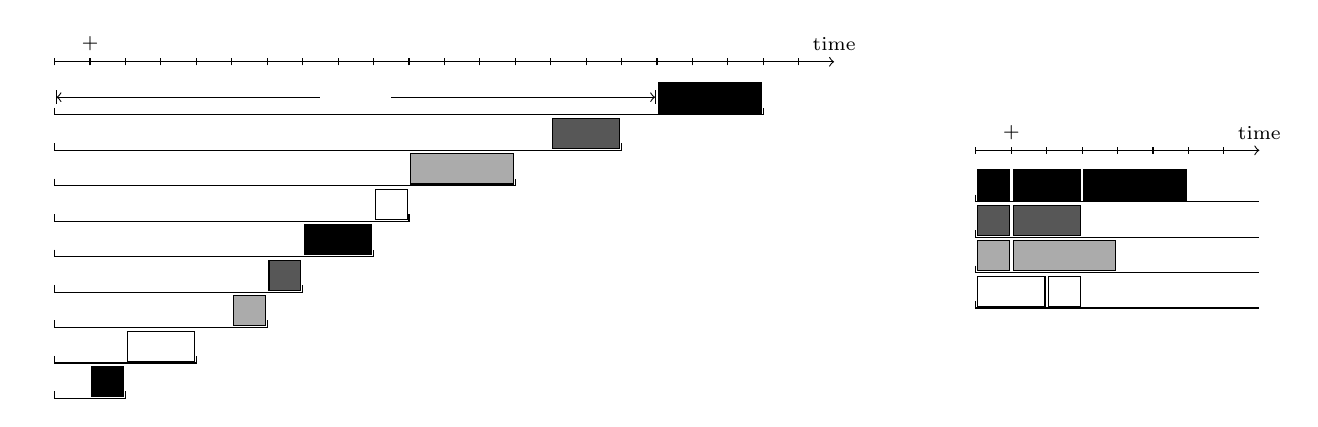
\begin{tikzpicture}[scale=0.45]
\newcounter{x}
  \newcommand\job[3]{
    \addtocounter{x}{1}
    \begin{scope}[shift={(0,-\value{x})}]
      \filldraw[fill=black!#3, shift={(-0.05,0)}] (#1.1,0.05) rectangle (#2,0.9);
      \draw (0,0.2) -- (0,0) -- (#2,0) -- +(0,0) -- +(0,0.2);
      \node at (-0.5,0.5) {\scriptsize{}};
    \end{scope}
  }
  \job{17}{20}{100}
  \job{14}{16}{66}
  \job{10}{13}{33}  
  \job{9}{10}{0}  
  \job{7}{9}{100}  
  \job{6}{7}{66} 
  \job{5}{6}{33} 
  \job{2}{4}{0}
  \job{1}{2}{100}
\node at (23,-4.5) {\LARGE{}};  
\draw[->] (0,0.5) -- (22,0.5);
\foreach \tick in {0,...,21}
    \draw (\tick,0.4) -- (\tick,0.6);
  \node at (0,1) {\scriptsize{}};
  \node at (1,1) {\scriptsize{+}};     
  \node at (22,1) {\scriptsize{time}};  
  \node at (20.7,-1) {\scriptsize{}};
  \node at (18.5,-0.57) {\textcolor{white}{\scriptsize{}}};
  \draw[<-] (0.05,-0.5) -- (7.5,-0.5);
  \draw[->] (9.5,-0.5) -- (16.95,-0.5);
  \draw (0.05,-0.3) -- (0.05,-0.7);
  \draw (16.95,-0.3) -- (16.95,-0.7);
  \node at (8.5,-0.5) {\scriptsize{}}; 
  
  \newcommand\sjob[7]{
      \filldraw[fill=black!#3, shift={(-0.05,0)}] (#1.1,-#4.05) rectangle (#2,-#4.9);
      \node at (#5,-#4.5) {\textcolor{black!#7}{\scriptsize{}}};
  }
  \begin{scope}[shift={(26,-2.5)}]
    \draw[->] (0,0.5) -- (8,0.5);
    \foreach \tick in {0,...,7}
      \draw (\tick,0.4) -- (\tick,0.6);
    \foreach \y/\machine in {0/1,1/2,2/3,3/4}{   
      \node at (-0.7,-\y.5) {\scriptsize{}}; 
      \draw[shift={(0,0.05)}] (0,-\y.8) -- (0,-\machine) -- (8,-\machine);
    }
    \node at (0,1) {\scriptsize{}};
    \node at (1,1) {\scriptsize{+}};     
    \node at (8,1) {\scriptsize{time}};        
    \sjob{0}{1}{100}{0}{0.5}{9}{0}
    \sjob{1}{3}{100}{0}{2}{5}{0}
    \sjob{3}{6}{100}{0}{4.5}{1}{0}
    \sjob{0}{1}{66}{1}{0.5}{6}{0}
    \sjob{1}{3}{66}{1}{2}{2}{0}
    \sjob{0}{1}{33}{2}{0.5}{7}{100}
    \sjob{1}{4}{33}{2}{2.5}{3}{100}
    \sjob{0}{2}{0}{3}{1}{8}{100}
    \sjob{2}{3}{0}{3}{2.5}{4}{100}            
  \end{scope}            
\end{tikzpicture} \caption{Visualization of jobs in set  and their  (temporal) distribution over machines. Left: Time window of each job with its processing volume pushed to the right. Right: resulting job-to-machine~assignment. Assume  to be small enough that none of the jobs gets safe before completion as well as  (the machines are called ).
}
\label{mp-fig: main-alg}
\end{figure}
\end{footnotesize}

Consider an arbitrary . By construction, we could feasibly schedule this set of jobs on a single machine using . However, doing so may completely use up the laxity of some job in , causing problems when new jobs are released in the future. We want to keep a constant fraction  (independent of ) of the initial laxity  for each  by distributing them carefully over  machines. Consider again  and assume an increasing order by deadlines. We further partition  into  different subsets  by setting  and schedule {\em each} of them on a separate machine via . By the right choice of , this reduces the decrease in laxity sufficiently. The procedure is visualized in Figure~\ref{mp-fig: main-alg}.

We know from the preliminaries that \EDF on  requires  machines. Hence the algorithm uses  machines. In Subsection~\ref{subsec: oa-analysis}, we prove that we can choose  so that a constant  as above exists and that , . The key to prove that lies in Subsection~\ref{subsec: oa-pow-lax} where we characterize the relation between a decrease in the laxity and increase in the number of machines. Hereby, we use the compact representation of the optimum value presented in Subsection~\ref{subsec:optimum}. In summary we need  machines. 

\subsection{Strong Density -- A Compact Representation of the Optimum}
\label{subsec:optimum}

The key to the design and analysis of online algorithms are good lower bounds on the optimum value. The offline problem is known to be solvable optimally in polynomial time, e.g., by solving a linear program or a maximum flow problem~\cite{horn74}. However, these techniques do not provide a quantification of the change in the schedule and the required number of machines when the job set changes. We derive an exact estimate of the optimum number of machines as an expression of workload that must be processed during some (not necessarily consecutive) intervals.





Let~ denote a set of  pairwise disjoint intervals~. We define the {\em length} of  to be  and its {\em union} to be . 

\begin{definition}[Strong density]
  Let  be as above and  be the feasible time window of job . The contribution  of job~ to  is the least processing volume of~ that must be scheduled within  in any feasible schedule, i.e.,

The strong density  is defined as maximum total contribution of all jobs over all interval sets:

\end{definition}






Our main result in this section is that  is the exact value of an optimal solution. We give a combinatorial proof, but we also note that it follows from LP duality.
\begin{theorem}
\label{thm: strong-density}

\end{theorem}
\begin{proof}
It is easy to see that  is a lower bound on  since the volume of  must be scheduled in  of length . This yields a lower bound of  for any .

It remains to show that . Given a schedule, we denote by  the number of time slots  during which exactly  machines are occupied. For any feasible schedule that uses  machines, we obtain a vector . We define a lexicographical order  on these vectors: we have  if and only if there exists some  with  and , for all . We pick the schedule whose corresponding vector is the smallest with respect to .

We now construct a directed graph  based on the schedule we pick. Let  where  represents the slot .
Let  be the number of machines occupied during . An arc from  to  exists iff  and there exists some job  with  whereas  is processed in  but not in .
Intuitively, an arc from  to  implies that one unit of the workload in  could be carried to .

We claim that in  there is no (directed) path which starts from some  with , and ends at some  with . Suppose there exists such a path, say  with  and . Then we alter the schedule such that we move one unit of the workload from  to , for all . By doing so,  decreased and  increased by  each. By  and , we get that  decreases by , contradicting the choice of the schedule.

Consider  and let  be the set of vertices reachable from  via a directed path (trivially, ). The above arguments imply that for any , it holds that . We claim that  for . Note there is no arc going out from  (otherwise the endpoint of the arc is also reachable and would have been included in ), i.e., we cannot move out any workload from , meaning that the contribution of all jobs to  is included in the current workload in , i.e., . Thus, 
Notice that  is either  or , and among them there is at least one of value , thus the right-hand side is strictly larger than , which implies that .  
\end{proof} 

\subsection{The Power of Laxity} \label{subsec: oa-pow-lax}

Let  be an arbitrary instance and  be rational. We analyze the influence that  the decrease in the laxity of each job by a factor of  has on the optimal number of machines. To this end, let  be the modification of  where we increase the processing time of each job by a -fraction of its initial laxity, i.e.,  and  (or equivalently ). Using a standard scaling argument, we may assume w.l.o.g.~that for a fixed  all considered parameters are integral.

Obviously, we have . In the following, we show  for instances  only consisting of sufficiently tight jobs.

\begin{theorem}\label{thm:laxity-drop} For every  consisting only of -tight jobs and , it holds that

\end{theorem}

In fact, we even show a slightly stronger but less natural result. More specifically, we split each job  into two subjobs: the \textit{left part} of , denoted , and the \textit{right part} of , denoted , where 

i.e., we split the former feasible time window at  and distribute  over both emerging jobs in such a way that the right part has the processing time of the original job . The sets containing all of these subjobs are  and , respectively. In the following, we show Theorem~\ref{thm:laxity-drop} even for  instead of . This implies, as can be easily seen, the statement for .

In the proof, we define two more jobs based on  and , namely the {\em -right-shortened} and the {\em -left-shortened} variant of , denoted  and  and contained in the sets  and , respectively. We define

which means that we drop an amount of  from either side of the feasible time window while keeping the processing time. We then show the following lemma.

\begin{figure}
\centering
\definecolor{light-gray}{gray}{0.7}
\begin{tikzpicture}[scale=0.35]
  \newcommand\poljob[5]{
    \begin{scope}[shift={(#3,#4)}]
      \filldraw[fill=black!70, shift={(-0.05,0)}] (#1,0.05) rectangle (#2,0.9);
      \draw (0,0.2) -- (0,0) -- (#2,0) -- +(0,0) -- +(0,0.2);
      \node at (-0.5,0.5) {\tiny{#5}};
    \end{scope}
  }
  \newcommand\mpoljob[6]{
    \begin{scope}[shift={(#3,#4)}]
      \draw[draw=black!30] (0,0.2) -- (0,0) -- (10,0) -- +(0,0) -- +(0,0.2);    
      \filldraw[fill=black!70, shift={(-0.05,0)}] (#1,0.05) rectangle (#2,0.9);
      \draw (#6,0.2) -- (#6,0) -- (#2,0) -- +(0,0) -- +(0,0.2);
      \node at (-0.85,0.5) {\tiny{#5}};
      \node at (10,-0.5) {\textcolor{light-gray}{\tiny{}}};
      \node at (0,-0.5) {\textcolor{light-gray}{\tiny{}}};        
    \end{scope}
  }  
  \poljob{6.1}{10}{0}{0}{}
  \poljob{3.1}{10}{0}{-4}{}
  \mpoljob{1.6}{4.5}{-12}{-8}{}{0}\mpoljob{6.1}{10}{12}{-8}{}{4.5}\mpoljob{1.6}{5.5}{-12}{4}{}{0}\mpoljob{6.1}{10}{12}{4}{}{4.5}

  \draw[<-] (0.05,0.5) -- (2,0.5);
  \draw[->] (4,0.5) -- (5.95,0.5);
  \draw (0.05,0.7) -- (0.05,0.3);
  \draw (5.95,0.7) -- (5.95,0.3);
  \node at (3,0.5) {\tiny{}};     
  \node at (8,0.43) {\textcolor{white}{\tiny{}}};
  \node at (10,-0.5) {\tiny{}};
  \node at (0,-0.5) {\tiny{}};
  
  \draw[->, decorate, decoration={snake, amplitude=1.5pt}] (5,-0.2) -- (5,-2.9);
  \node[align=center] at (6.5,-1.5) {\tiny \begin{tabular}{c}drop\\ laxity\end{tabular}};
  
  \draw (5,-4.2) edge[out=270,in=180,->,looseness = 0.8] (10.5,-7.5);
  \draw (5,-4.2) edge[out=270,in=0,->,looseness = 0.8] (-0.5,-7.5);
  \node at (5,-6.5) {\tiny{split}};
   
  \draw[->] (5,1.2) -- (10.5,3.5);
  \node[align=center] at (9.5,2) {\tiny shorten left};  
  
  \draw[->] (5,1.2) -- (-0.5,3.5);
  \node[align=center] at (0.1,2) {\tiny shorten right};    
  
  \draw[->,dashed] (-10,3) -- (-10,-6);
  \node[align=center] at (-12,-2) {\tiny \begin{tabular}{c}strictly\\ harder\\ for \end{tabular}};  
  
  \draw[<->,dashed] (19,3) -- (19,-6);
  \node[align=center] at (21,-2) {\tiny \begin{tabular}{c}identical\\ for \end{tabular}};             
\end{tikzpicture} \caption{The different types of jobs defined for the proof of Theorem~\ref{thm:laxity-drop} and their relations. We let  and }
\label{fig: power-lax}
\end{figure}

\begin{lemma}\label{lemma:laxity-release-increase}
For every  and , it holds that

\end{lemma}
\begin{proof}
We representatively show the statement for ; the argumentation for  is analogous. According to Theorem~\ref{thm: strong-density}, there exists a set of  pairwise disjoint intervals  such that 
W.l.o.g, we assume that  with  where  (hence, ), for all . To derive the relationship between  and , we expand  into a set of element-wise larger intervals  such that . We show for each job  that  and thus the lemma follows.

The expanding works as follows. Given  as above, we expand each of the intervals  to  with  the following way. We start at the rightmost interval  and try to set  for . If this would, however, produce an overlap between  and , we set ,  and try to additionally expand  by  instead. After that, we continue this procedure to the left but never expand an interval into negative time. More formally, we let~  and set for all  

The following two facts can be easily observed.

\begin{observation}\label{lemma:expand-length}
Consider  as above. One of the following statements is true:
\begin{enumerate}[(i)]
  \item We have  and .
  \item We have  and .
\end{enumerate}
\end{observation}

\begin{observation}\label{lemma:expand-subintervals}
If , then .
\end{observation}






We now consider any job  with  and claim that . First plug in the definition of contribution. We get

It thus suffices to prove that .

Let  where we let  be the leftmost point of it and  be the rightmost one. By Observation~\ref{lemma:expand-subintervals}, it follows that , i.e., we can restrict to proving  According to Observation~\ref{lemma:expand-length}, there are two possibilities. 

\noindent\textbf{Case 1.} We have . Given the fact that  and , it follows that . 

\noindent\textbf{Case 2.} It holds that  takes up a length of  in the interval  Hence for any , it takes up a length of at least  in the interval . Using , we get . Thus, if we let , we get that  takes up a length of at least  in the interval . Since , we have , which completes the proof.
\end{proof}



\begin{proof}[Proof of Theorem~\ref{thm:laxity-drop}.]
We show that  or, more specifically, that . 

For the first part, compare the two instances  and . We observe that  for all , where we use for the first part that  is -tight. This implies that a schedule of  on  machines can be easily transformed into a schedule of  on  machines. Hence, we get that  and the claim follows by Lemma~\ref{lemma:laxity-release-increase}.

For the second part, we simply observe that  and apply Lemma~\ref{lemma:laxity-release-increase} again.
\end{proof}

\subsection{Analysis} \label{subsec: oa-analysis}

For the sake of simplicity, we choose  such that  is integral. We now analyze the performance of our algorithm. The goal of this subsection is proving the following theorem.

\begin{theorem}\label{thm:logn}
Our algorithm is an -competitive algorithm for the machine minimization problem.
\end{theorem}

Recall that we apply \EDF to schedule the safe jobs . Using Theorem~\ref{thm: EDF-small},  machines are suffice to feasibly schedule all the safe jobs. Meanwhile at any time , we partition  into  subsets  and schedule  jobs of each subset on a separate set of machines.

We first prove that, if we choose a certain , the laxity of each job in  never drops below a constant fraction of its original laxity. This implies that our algorithm never misses a critical job. Hence our algorithm does not miss any job.

\begin{lemma}\label{lemma:length-preempted}
We can choose  such that at any time  and for any ,  where .
\end{lemma}
\begin{proof}
Let  be an arbitrary time when the partition of  into the sets  is recomputed. Let  and w.l.o.g.  where , for all . By the way the partition is constructed, we further have . Now let  and notice that, unless the partition is recomputed, the execution of  is only blocked by other jobs for at most  (if  does not exist,  is immediately executed). Since every job in  is -tight at , this however means that the execution of  is only delayed by . Note that we can choose  in such a way that . To get the total time  is at most delayed by, we have to sum over all such . Recall that at least one job is released at any such time , hence  and we have: \end{proof}

Before proving the main theorem, we need an additional bound on . To this end, let  be the set of residues of  at , i.e., the jobs in  with remaining processing times and time windows.

\begin{lemma}\label{lemma:partition-at-time-t} At all times , it holds that

\end{lemma}

W.l.o.g., we let  where , for all . We first prove the following auxiliary lemma:

\begin{lemma}\label{lemma:length-shrink}
For any  and , we have .
\end{lemma}
\begin{proof}
Suppose there exists some  such that  holds for any h with . Given that every job in  is -tight at , we get . Thus, the total workload that has to be finished in the interval  is larger than , which contradicts the fact that  machines are enough to accommodate .
\end{proof}

\begin{proof}[Proof of Lemma~\ref{lemma:partition-at-time-t}]
Recall the construction of the different  and consider the state of  when  is opened. Then there exists some job  which could not be added into any of the subset  to . As before, we let  be the earliest-deadline job from . Obviously job  is added to  before we consider job , . According to Lemma~\ref{lemma:length-shrink}, there are at least  jobs among  whose feasible time window has a length at least , and has a remaining laxity no more than . Thus if we consider the interval , each of the  contribute at least a processing time of , implying that the workload that has to be finished in this interval is at least . On the other hand, as  machines are enough to accommodate all the jobs, the workload processed during  is at most . Hence , which implies the lemma.
\end{proof}

We are ready to prove the main theorem of this section:

\begin{proof}[Proof of Theorem~\ref{thm:logn}.]
Recall that the number of machines used by our algorithm is . Using Lemma~\ref{lemma:length-preempted}, it only remains to bound  and . We set . 

We first show  for all . According to Lemma~\ref{lemma:partition-at-time-t}, it suffices to prove that . By Lemma~\ref{lemma:length-preempted}, we know that for any job , we have . Consider the instance  as defined in Subsection~\ref{subsec: oa-pow-lax}. Any feasible schedule of  implies a feasible schedule of , i.e., we get . Theorem~\ref{thm:laxity-drop} implies that  and the claim follows.

Moreover, we show . Consider any job . If job  is released at time , then . Otherwise  we have  according to Lemma~\ref{lemma:length-preempted}. As  is -tight at  and becomes -loose at , it follows that  is processed in , implying that . Thus it holds that . As a consequence, any feasible schedule of  implies a feasible schedule of , implying that  by Theorem~\ref{thm:laxity-drop}.
\end{proof}





\section{Lower Bounds}
\label{sec:LB}

\subsection{Lower bound for \LLF}

Phillips et al.~\cite{phillipsSTW02} showed that the competitive ratio of \LLF for (semi-)online machine minimization is not constant. We extend their results by showing that \LLF requires  machines.


\begin{theorem}\label{thm:LLF-lower-bound}
  There exists an instance of  jobs with a feasible schedule on  machines for which \LLF requires  machines.
\end{theorem}
\begin{proof}
Let  be even. For any , we give an instance at which \LLF using  machines fails. Towards this, consider the integer sequence  with  large enough and , for all . Let  be the set of  identical {\em (more tight)} jobs with feasible time window  and laxity . Moreover, let  be the set of  identical {\em (more loose)} jobs with feasbile time window  and processing time . We construct the instance in  rounds (where  is yet to be specified) as follows.

\begin{itemize}
\item {\em Round 1.} From time  to time , we release  and  for  where . It can be easily verified that \LLF will always preempt jobs in  in favor of jobs in . Thus at time , each job in  is preempted for exactly  time units, i.e., by time  there are still  jobs in , each having a remaining processing time of  to be scheduled within . However, the optimum solution could finish all the jobs released so far by time . 

\item {\em  Round .} Carry on the above procedure. Suppose at time  the optimum solution could finish all the jobs released so far while for \LLF there are still  jobs, each having a remaining processing time  to be scheduled within . Then from time  to time , we release  and  for  where .
It can be easily seen that at time  there are in total  jobs having a processing time  to be scheduled within . Each of these jobs will be preempted in favor of jobs in . Thus until time , it is preempted for  time units. This implies that there are  jobs, each having a processing time  to be scheduled within . However, the optimum solution could finish all the jobs released so far by time .
\end{itemize}

We estimate the number of jobs released at each round by . Thus, until round  we release in total  jobs. It is easy to see that \LLF requires  machines for the remaining jobs and  machines will be insufficient if we choose some . Thus it suffices to choose some  for the lower bound, i.e., \LLF requires  many machines.
\end{proof}

\subsection{Lower bound for Deadline-Ordered Algorithms}

Consider deadline-ordered algorithms that schedule jobs using only the relative order of jobs instead of their actual values. \EDF belongs to this class of algorithms. Lam and To~\cite{lamT99} derived a lower bound on the speed that is necessary to feasibly schedule jobs on~ machines. We modify their instance and argumentation to give the following lower bound on the number of unit-speed machines.

\begin{theorem}\label{thm:deadline-ordered}
  There are instances of~ jobs with a feasible schedule on~ machines for which any deadline-ordered algorithm requires at least~ machines.
\end{theorem}

\begin{proof}
We define a collection of instances with identical job sets that all can be feasibly scheduled on~ machines. The only difference in the instances are the deadlines but the relative order is again the same. Thus, a deadline-ordered algorithm cannot distinguish the instances and must produce the same schedule for all of them. We show that this property enforces that (nearly) each job must run on its own machine.

For each~ we define the job set~ as follows:


For every instance~, , there is a feasible solution on  machines. Schedule the first  jobs in order of their indices one after the other filling a machine up to the deadline~ before opening the next machine. Since every job has a processing time less than~, no job will run simultaneously on more than one machine. The total processing volume is 

and thus, all jobs are feasibly scheduled on  machines. The remaining jobs are scheduled by the same procedure in the interval . With a similar argumentation as above, this is a feasible schedule. In particular, the total processing volume is


We now show that any fixed schedule  must use~ machines to guarantee a feasible solution for all instances~. With the argumentation above this implies the lower bound for any deadline-ordered algorithm. 

W.l.o.g.~we may assume that the order of job indices is the order of deadlines. We could enforce this explicitly by adding a small value, but omit it for the sake of presentation. 

Any deadline-ordered solution must complete the first  jobs by time~ to be feasible for~ for~. Since in any instance~ the largest among those jobs has processing time , each job with index  must receive its exclusive machine. That means, we need~ machines for jobs~. The remaining~ jobs with unit processing time must finish in instance~ by time~ which requires~ machines. In total, a deadline-ordered algorithm needs~ machines whereas optimal solutions with~ machines exist.
\end{proof}

Notice that this very fatal lower bound is achieved already by instances in which all jobs are released at the same time.  Thus, it is not the lack of information about further job arrivals but the lack of precise deadline information that ruins the performance.

\section{Concluding Remarks}

We contribute new algorithmic results for a fundamental online resource minimization problem. We give the first constant competitive algorithms for a major subclass in which jobs have agreeable deadlines, 
and also improve on upper bounds for the general problem. It remains as a major open question if the general preemptive problem admits a constant competitive ratio. We believe that some of our techniques may be useful for the closely related online throughput maximization problem, where we relax the requirement that all jobs must be scheduled (and fix a number of machines). It would also be interesting to quantify the tradeoff between the number of machines and the guaranteed~throughput.


\section*{Acknowledgment} We thank Naveen Garg for discussions on deadline-ordered algorithms and his contribution to the lower bound in Theorem~\ref{thm:deadline-ordered}. Moreover, we thank Benjamin Müller for interesting discussions at an early stage of the project. As part of his Master's thesis he contributed to Thm.~\ref{thm: black box} and part of Thm.~\ref{thm:preempt-samesize-optunknown}.

\bibliographystyle{abbrv}
\bibliography{machinenum}


\end{document}